% Signal-MC shape material; figures are regenerated from the pinned v6.4 inputs.
% The root report supplies the preamble and the running figure counter.
\clearpage\section*{2016 signal MC: where does the reconstructed core lie?}

\textbf{The result.} The supplied 2016 signal histograms have a small downward core displacement over 40--175 MeV: the fitted center is 0.08--1.02 MeV below the generated mass. The sign agrees with the saved 2021 samples, but the displacement is smaller. The selected distributions also have measurable non-Gaussian tails. These observations motivate using each year's own MC shape and core location in the extraction that follows.

\textbf{Inputs.} The 29 ROOT files contain 3,770,135 selected entries at generated masses from 30 to 175 MeV, in nominal 5 MeV steps; the 150 MeV sample is missing. The analyzed histogram is \texttt{h\_MinvScSm\_GeneralLargeBins\_Final\_1}. According to the supplied sample description, it contains prompt target-constrained signal with FEE momentum scaling and smearing already applied. No additional smearing is applied here. The unsmeared histogram is inventoried but is not used to determine the template.

\begin{center}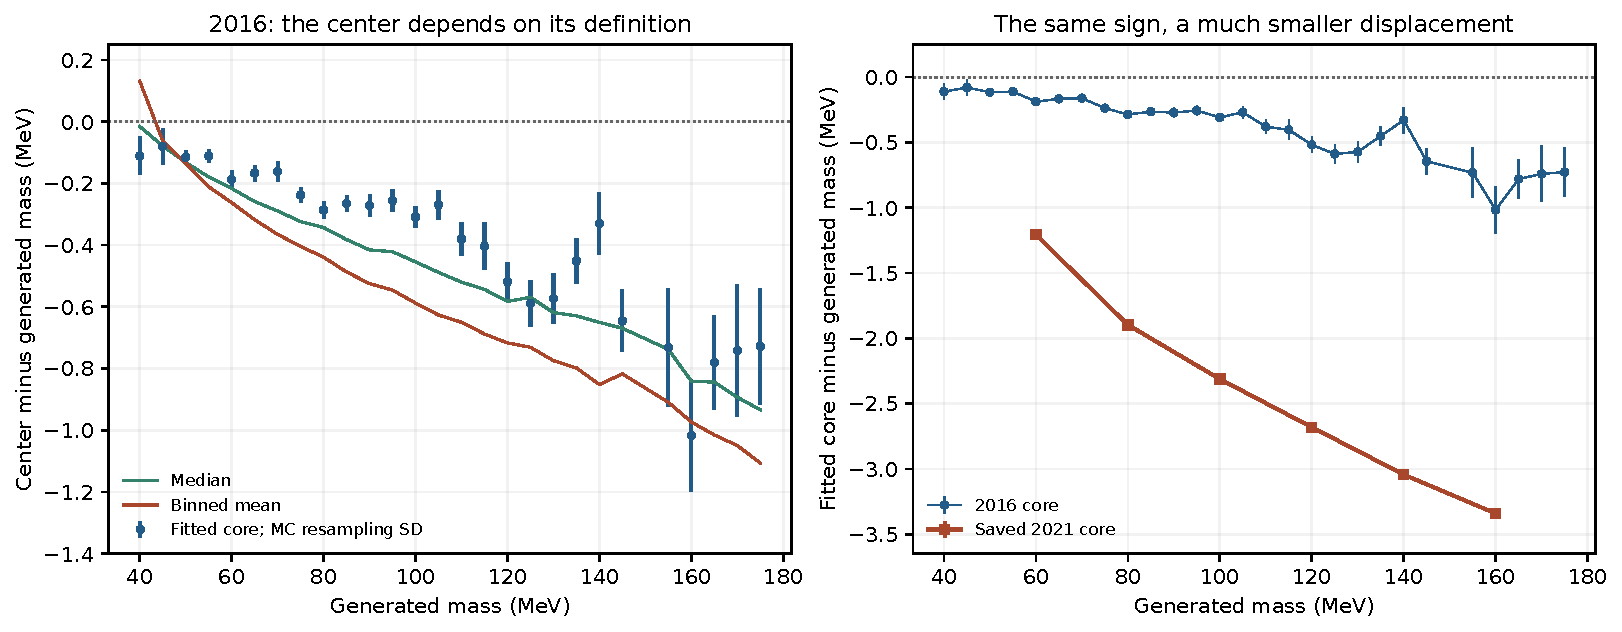
\includegraphics[width=\linewidth,height=3.3in,keepaspectratio]{../figures/shape_centers_and_2021.pdf}\end{center}
{\small\refstepcounter{figure}\textbf{Figure \thefigure. How to read the figure.} Left: the fitted core, median and binned mean answer different location questions because the distributions have tails. Right: the 2016 core locations are compared with the earlier v6.1 2021 results using the same local-core convention. The extraction later uses the separate latest v16 TC bank. Bars are the standard deviation over MC bin-resampling fits: 64 replicas for 2016 and 32 for 2021. They describe finite-MC variation, not detector calibration uncertainty. Reconstruction and selection equivalence between the two sets of samples has not been established.}\par\medskip

\begin{center}\small\begin{tabular}{rrrr}\toprule
Generated mass [MeV] & 2016 core [MeV] & Shift [MeV] & MC SD [MeV]\\\midrule
60 & 59.812 & $-0.188$ & 0.028\\
100 & 99.691 & $-0.309$ & 0.034\\
160 & 158.983 & $-1.017$ & 0.181\\
\bottomrule\end{tabular}\end{center}

The fitted core locates the main peak. The median divides the full selected probability in half. The mean includes the entire tail and can move when a small amount of probability lies far from the peak. The core is the location used to align templates; the mean and median remain useful independent descriptions. The 30 and 35 MeV samples require separate treatment below, so the primary template domain begins at 40 MeV.

\clearpage\section*{How are the core center and width defined?}

The locator follows the convention used for the signal-MC comparisons in v6.3.6. It finds a smoothed mode within three reference analysis widths of the generated mass, then fits the unsmoothed bins within 1.5 reference widths of that mode. The model is a bin-integrated Gaussian plus a nonnegative affine pedestal, fitted by Poisson deviance. The pedestal describes the broad signal shoulders locally; it is not a collision-background component.

\begin{center}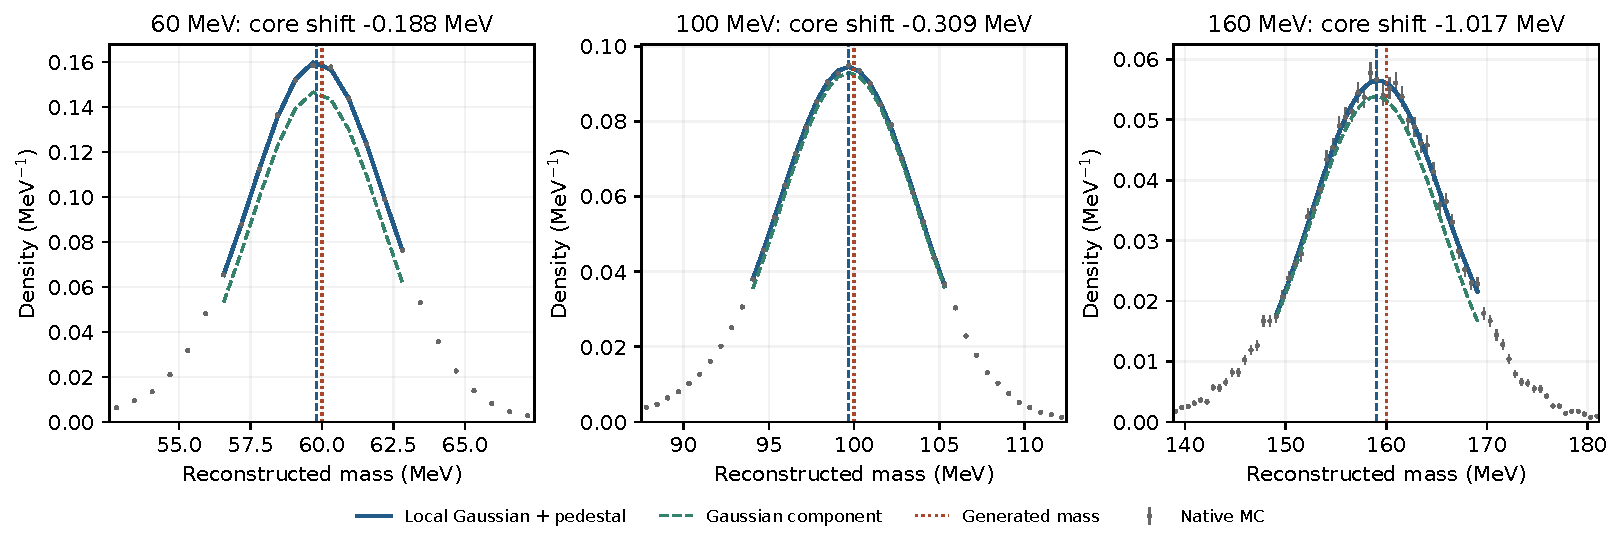
\includegraphics[width=\linewidth,height=2.0in,keepaspectratio]{../figures/shape_core_fit_examples.pdf}\end{center}
{\small\refstepcounter{figure}\textbf{Figure \thefigure. How to read the figure.} Points are the native 0.625 MeV bins, with square-root-count bars. Blue: the local Gaussian plus pedestal, drawn only across its fitted bins. Green: its Gaussian component. The red vertical line is the generated mass; the blue dashed line is the fitted core. Integrating the model over each bin avoids defining the center by the tallest bin alone.}\par\medskip

\begin{center}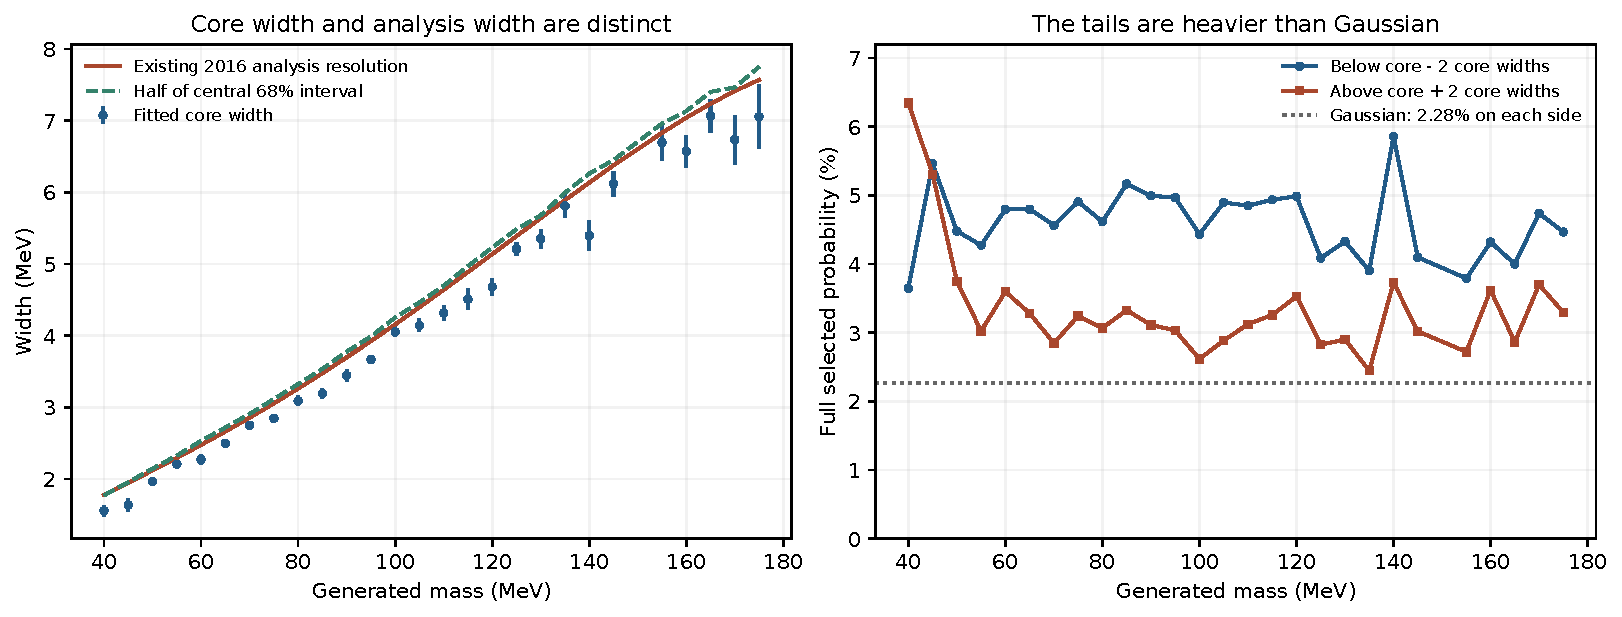
\includegraphics[width=\linewidth,height=2.05in,keepaspectratio]{../figures/shape_widths_and_tails.pdf}\end{center}
{\small\refstepcounter{figure}\textbf{Figure \thefigure. How to read the figure.} Left: fitted core width, existing 2016 analysis-resolution curve, and half the central 68\% probability interval. These are distinct width definitions. Right: full selected probability below and above two fitted core widths. A Gaussian has 2.28\% on each side. Core-width bars are MC resampling standard deviations.}\par\medskip

The core width grows from 1.56 MeV at 40 MeV to 7.06 MeV at 175 MeV and is 0.84--0.99 times the reference analysis width. Between 89.2\% and 93.7\% of selected probability is within two core widths, compared with 95.45\% for a Gaussian. The reference-width curve helps define the locator; the new MC extraction instead uses the interpolated fitted core width to define its window.

All 1,728 resampling fits in the primary domain pass the locator checks. A separate definition test varies the fitting range and removes the pedestal. The largest center change at 60, 100 and 160 MeV is 0.044, 0.084 and 0.396 MeV. This spread is reported separately from the MC error: it shows that a precise statistical center can still depend on the local-fit definition.

\clearpage\section*{Overlay the distributions while retaining their tails}

\begin{center}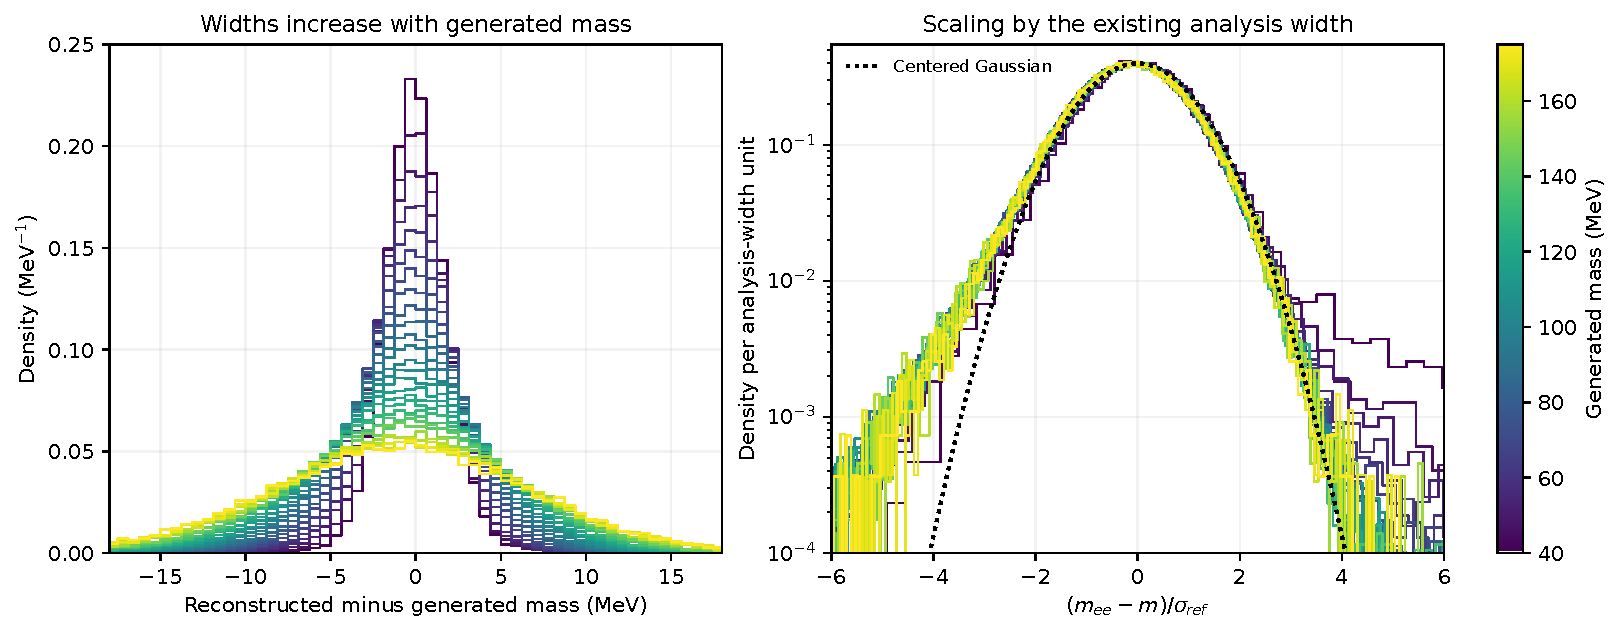
\includegraphics[width=\linewidth,height=3.05in,keepaspectratio]{../figures/shape_generated_aligned_overlays.pdf}\end{center}
{\small\refstepcounter{figure}\textbf{Figure \thefigure. How to read the figure.} Every colored curve is one native 2016 histogram divided by its own full selected count. Left: subtracting the generated mass leaves the growth in width visible. Right: scaling by the existing analysis width brings the curves closer together. The dotted Gaussian is centered at the generated mass. The logarithmic scale reveals tail differences. Neither panel renormalizes the displayed mass range.}\par\medskip

\begin{center}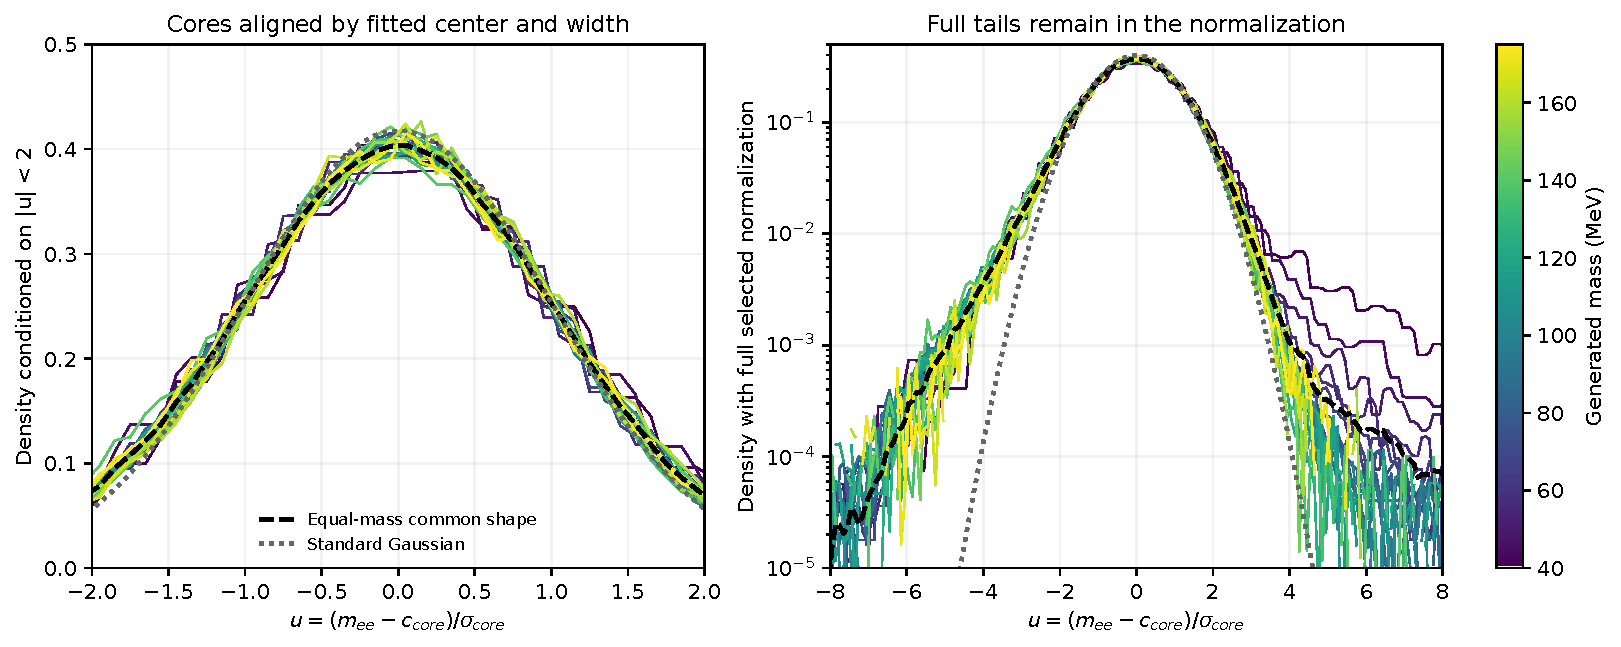
\includegraphics[width=\linewidth,height=3.05in,keepaspectratio]{../figures/shape_core_aligned_overlays.pdf}\end{center}
{\small\refstepcounter{figure}\textbf{Figure \thefigure. How to read the figure.} Here $u=(m_{\rm rec}-c)/s$, where $c$ and $s$ are each histogram's fitted core center and width. Left: each distribution is conditioned on $|u|<2$ to compare central shapes. Right: its full selected normalization is restored. The black dashed curve is an equal-mass average of the 27 aligned empirical distributions; the gray dotted curve is a standard Gaussian with the corresponding normalization.}\par\medskip

\textbf{Answer.} Alignment produces similar central shapes, but it does not make the complete distributions identical. Conditioning on the core hides differences in the amount of signal outside it. The full-distribution panel shows why a common core description can be useful while a mass-dependent MC template is still preferable for the selected signal yield.

\clearpage\section*{Use separate empirical centers for 2016 and 2021}

\textbf{The 2021 displacement should not be transferred to 2016.} At generated masses of 60, 100 and 160 MeV, the saved 2021 core shifts are $-1.208$, $-2.312$ and $-3.342$ MeV. The corresponding 2016 shifts are $-0.188$, $-0.309$ and $-1.017$ MeV. Both the locations and the tail probabilities differ.

\begin{center}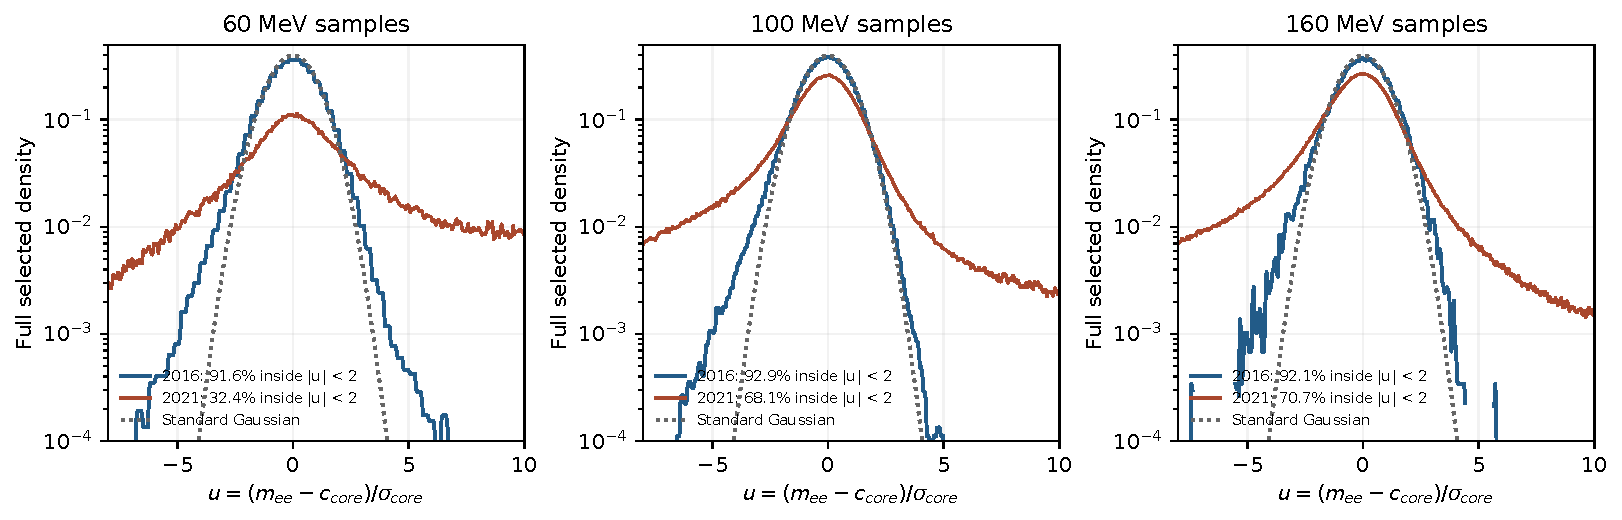
\includegraphics[width=\linewidth,height=3.25in,keepaspectratio]{../figures/shape_cross_year_shapes.pdf}\end{center}
{\small\refstepcounter{figure}\textbf{Figure \thefigure. How to read the figure.} Each year is aligned by its own fitted core center and width. Curves retain full selected normalization, including the saved 2021 overflow normalization. The percentages give the probability within $|u|<2$. The 2016 samples are more concentrated around their cores. This compares the supplied samples; it does not identify whether reconstruction, selection, calibration or another difference causes the change.}\par\medskip

For orientation, an equal-weight affine fit to the 2016 core shifts gives
\[
 c(m)=m-0.363673-0.563179\frac{m-100}{100},
 \qquad 40\le m\le175\ \mathrm{MeV},
\]
with all masses in MeV. Leaving out each mass in turn gives an RMS prediction error of 0.103 MeV and a largest absolute error of 0.351 MeV. This is a compact description of the trend. The extraction uses the empirical centers and their local interpolation instead, so it preserves the measured mass dependence without imposing this smooth law.

\textbf{The coordinate used by the MC method.} At a tested generated mass $m$, let $c_y(m)$ and $s_y(m)$ be the interpolated core center and width for year $y$. Then
\[
 u_y=\frac{m_{\rm rec}-c_y(m)}{s_y(m)}.
\]
The adopted 2016 fit and GP-training exclusion use $-3.5\le u_{2016}\le+3.5$. The 2021 method retains $-4\le u_{2021}\le+3$. Thus each window follows its own reconstructed MC core. The tested mass remains the generated signal mass, and is the horizontal coordinate of the limit and local-probability scans.

These shifts describe selected MC after its stated scaling and smearing. They do not establish a data mass-scale correction or identify the physical cause of the displacement. The saved 2021 signal-MC reference is the same input used for the introductory shape comparisons in v6.3.6.

\clearpage\section*{Why use the neighboring MC templates?}

\textbf{The comparison.} A Gaussian at the measured core, a common aligned empirical shape, and interpolation of the nearby samples are compared with the native histograms. For the common shape and neighbor tests, the tested histogram is omitted when constructing the approximation. The neighbor method must predict its center and width as well as its standardized shape.

\begin{center}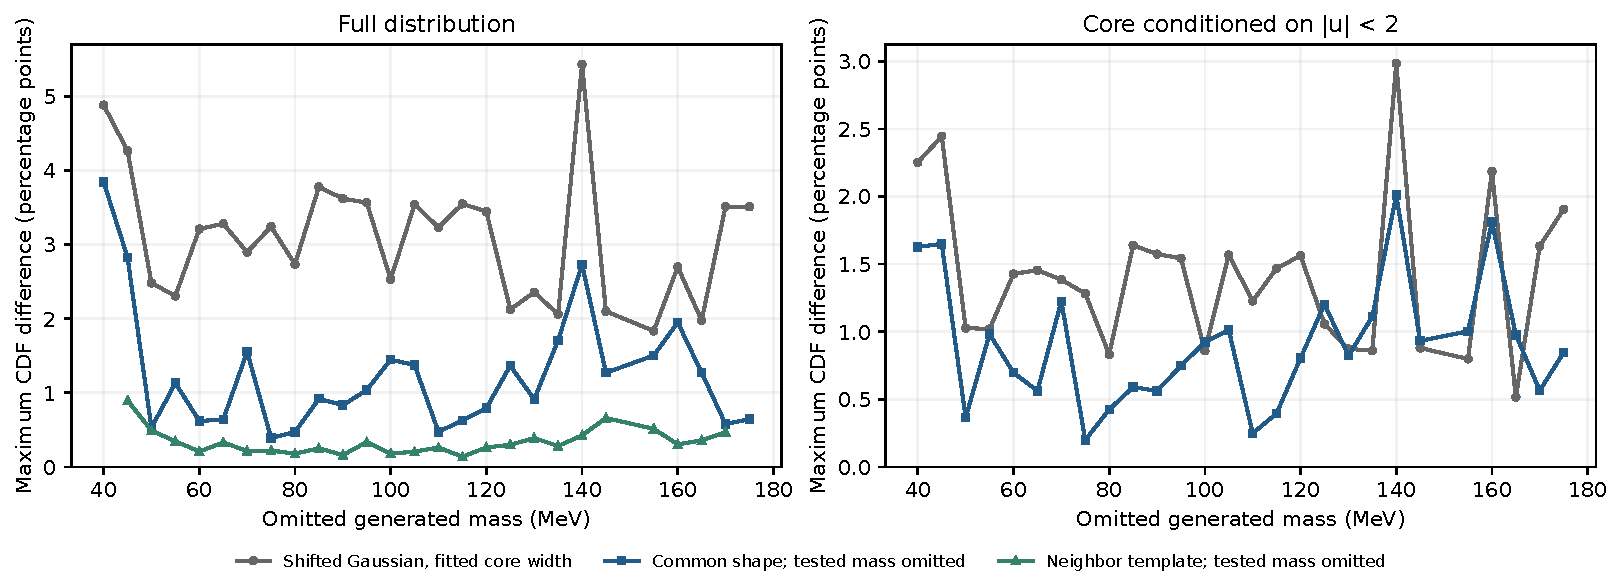
\includegraphics[width=\linewidth,height=3.2in,keepaspectratio]{../figures/shape_shape_holdout.pdf}\end{center}
{\small\refstepcounter{figure}\textbf{Figure \thefigure. How to read the figure.} The vertical axis is the largest absolute cumulative-probability difference, in percentage points: at native bin boundaries for the full distribution, and on a common standardized grid for the core. A value of one means that the integrated probabilities differ by one percentage point at some bin boundary. It is a shape discrepancy, not a $p$-value. The neighbor curve uses linear interpolation of both core center and width, as in the new extraction. Core-only comparisons condition on $|u|<2$ and use the measured center and width.}\par\medskip

\begin{center}\small\begin{tabular}{lrrr}\toprule
Full-distribution approximation & Median difference & Range & Tests\\\midrule
Gaussian at measured core & 3.23 pp & 1.83--5.43 pp & 27\\
Gaussian at full mean and RMS & 2.05 pp & 1.54--8.10 pp & 27\\
Common shape, tested mass omitted & 1.04 pp & 0.39--3.84 pp & 27\\
Neighbor template, tested mass omitted & 0.30 pp & 0.14--0.90 pp & 25\\
\bottomrule\end{tabular}\end{center}

\textbf{The adopted template.} At a simulated mass, use the native histogram. Between two simulated masses, linearly interpolate their core centers and core widths, align both histograms in $u$, and mix their cumulative distributions with the same mass interpolation weights. Taking differences of the resulting cumulative probabilities gives the probability in every requested analysis bin. The full selected normalization is retained throughout; fitting a finite window does not redefine the total signal yield.

The 150 MeV shape is interpolated between 145 and 155 MeV, because no 150 MeV input exists. The 40 and 175 MeV endpoints have no two-sided omitted-mass test. The older v6.4 shape study interpolated the logarithm of the width; this revision uses the linear-width convention shared with the latest 2021 neighbor method. The plotted neighbor checks have been recalculated for that convention. Linear interpolation has a slightly larger median discrepancy (0.30 rather than 0.24 percentage points); it is adopted for a consistent convention across years, not as an improvement over logarithmic-width interpolation.

The neighbor template gives the closest agreement in these omitted-mass shape checks. Finite-MC variation contributes to every discrepancy. These checks support the template choice, but they do not by themselves calibrate background absorption, limit coverage, or an uncertainty band for arbitrary intermediate masses. Those are different questions from how accurately one selected MC distribution predicts another.

\clearpage\section*{The 2016 window and the low-mass exceptions}

\begin{center}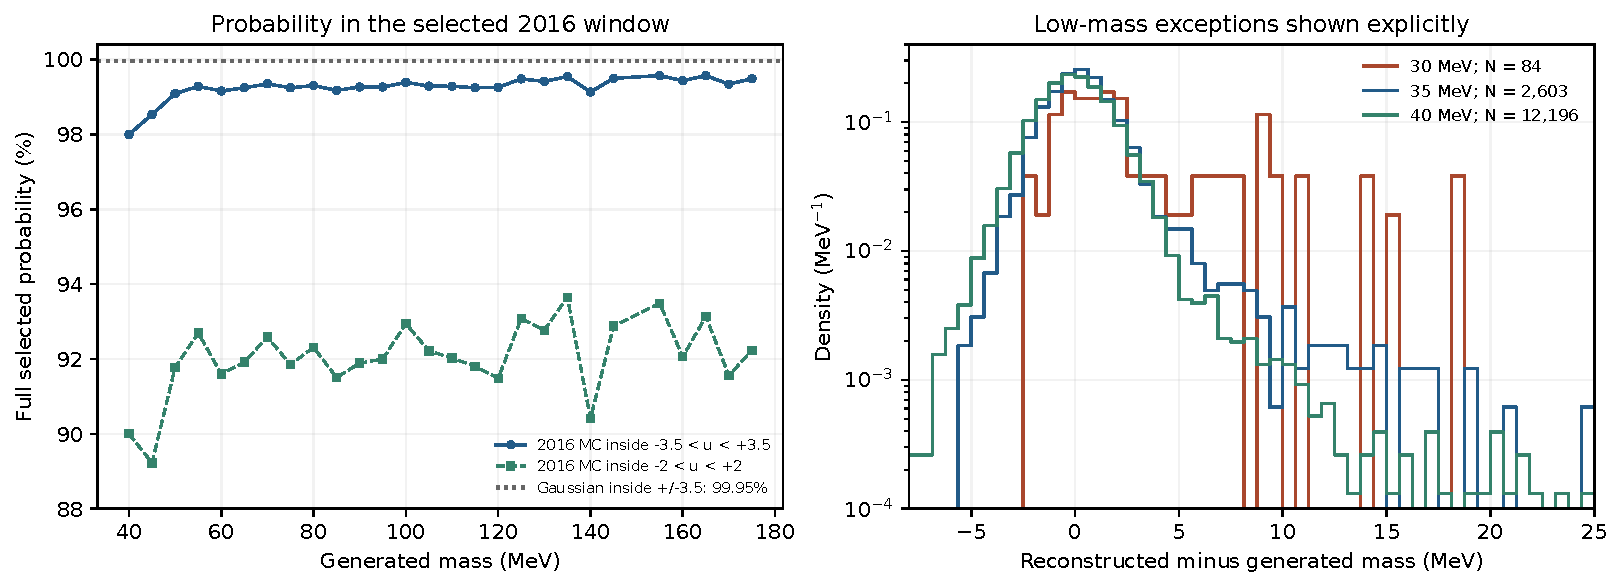
\includegraphics[width=\linewidth,height=3.3in,keepaspectratio]{../figures/shape_containment_and_low_mass.pdf}\end{center}
{\small\refstepcounter{figure}\textbf{Figure \thefigure. How to read the figure.} Left: the full selected probability inside $-3.5\le u\le+3.5$, the adopted 2016 fit and training-exclusion interval. The narrower $|u|<2$ fraction is a shape reference. A matched Gaussian has 99.95\% inside $|u|<3.5$. Right: the 30, 35 and 40 MeV histograms are shown without rescaling their displayed ranges. The two sparse low-mass samples are retained visibly rather than pooled into the primary shape comparison.}\par\medskip

The adopted window contains 98.00--99.57\% of the full selected MC probability across the primary 2016 samples. This is the geometric fraction of a signal template inside a specified interval. It is not a selection efficiency or a measured recovery fraction. Signal outside the excluded region can still enter the GP-training sidebands; a wider exclusion changes both the signal contamination and the available background information.

\textbf{30 MeV: no reliable fitted core.} Only 84 entries survive in the supplied histogram. The primary fit reaches its minimum-width bound, and only 34 of 64 resampling fits pass the locator checks. The binned mean is 34.10 MeV and the median is 31.81 MeV. Neither statistic makes the failed local Gaussian fit a reliable core measurement. Its attempted fit remains in the numerical ledger, but is not used for interpolation.

\textbf{35 MeV: a separate diagnostic.} This histogram has 2,603 entries. Its primary core center is 35.276 MeV and its mean is 35.695 MeV. Changing the pedestal-fit half-width from 1.5 to 2.0 reference widths changes the fitted core width from about 0.91 to 1.44 MeV. That sensitivity motivates keeping this sample outside the primary template prescription.

\textbf{40--175 MeV: the primary template domain.} All 27 available core fits and all their resampling fits pass. The 40 MeV sample remains in the comparison and has the largest common-shape discrepancy, so the low-mass qualification does not conceal the remaining shape change. No empirical template is extrapolated below 40 or above 175 MeV.

\textbf{Input checks.} Every analyzed histogram is a 400-bin TH1D on 0--0.25 GeV, converted once to 0--250 MeV. Its bins are 0.625 MeV wide; counts are nonnegative integers, variances equal counts, entries equal the bin sum, and underflow and overflow are zero. Generated masses come from the file names. The ROOT files have blank axis titles and no embedded fits; the supplied sample description provides the prompt/target-constrained and FEE provenance.

\clearpage\section*{Native central locations and widths}

All masses and widths are in MeV. Here $c$ is the fitted core center, SD is its conditional MC resampling error, $s$ is the fitted core width, and $F_2$ is the full selected fraction inside $c\pm2s$. ``Spread'' is the largest change in center across the four alternate local-fit definitions. The CSV retains more precision than this table.

\begin{center}\fontsize{8.5}{10.5}\selectfont\setlength{\tabcolsep}{3.1pt}
\begin{tabular}{rrrrrrrrrr}\toprule
$m$ & Entries & $c$ & $c-m$ & SD$(c)$ & $s$ & Median & Mean & $F_2$ [\%] & Spread\\\midrule
30 & 84 & -- & -- & -- & -- & 31.806 & 34.100 & -- & --\\
35 & 2,603 & 35.276 & $+0.276$ & 0.088 & 0.913 & 35.313 & 35.695 & 70.8 & 0.145\\
40 & 12,196 & 39.889 & $-0.111$ & 0.062 & 1.560 & 39.984 & 40.131 & 90.0 & 0.075\\
45 & 46,316 & 44.920 & $-0.080$ & 0.059 & 1.641 & 44.922 & 44.938 & 89.2 & 0.119\\
50 & 91,802 & 49.884 & $-0.116$ & 0.022 & 1.967 & 49.868 & 49.865 & 91.8 & 0.049\\
55 & 139,637 & 54.888 & $-0.112$ & 0.021 & 2.208 & 54.821 & 54.789 & 92.7 & 0.050\\
60 & 188,657 & 59.812 & $-0.188$ & 0.028 & 2.274 & 59.783 & 59.737 & 91.6 & 0.044\\
65 & 221,366 & 64.833 & $-0.167$ & 0.026 & 2.500 & 64.741 & 64.682 & 91.9 & 0.067\\
70 & 245,676 & 69.839 & $-0.161$ & 0.033 & 2.751 & 69.710 & 69.635 & 92.6 & 0.102\\
75 & 280,200 & 74.762 & $-0.238$ & 0.024 & 2.847 & 74.676 & 74.596 & 91.8 & 0.036\\
80 & 277,884 & 79.714 & $-0.286$ & 0.027 & 3.094 & 79.657 & 79.561 & 92.3 & 0.056\\
85 & 273,602 & 84.735 & $-0.265$ & 0.026 & 3.194 & 84.618 & 84.513 & 91.5 & 0.078\\
90 & 273,665 & 89.728 & $-0.272$ & 0.035 & 3.447 & 89.584 & 89.475 & 91.9 & 0.087\\
95 & 309,188 & 94.744 & $-0.256$ & 0.036 & 3.670 & 94.578 & 94.454 & 92.0 & 0.113\\
100 & 290,224 & 99.691 & $-0.309$ & 0.034 & 4.055 & 99.546 & 99.412 & 92.9 & 0.084\\
105 & 172,514 & 104.731 & $-0.269$ & 0.046 & 4.145 & 104.512 & 104.373 & 92.2 & 0.163\\
110 & 148,579 & 109.620 & $-0.380$ & 0.053 & 4.317 & 109.480 & 109.350 & 92.0 & 0.061\\
115 & 124,340 & 114.596 & $-0.404$ & 0.076 & 4.510 & 114.456 & 114.312 & 91.8 & 0.082\\
120 & 114,544 & 119.481 & $-0.519$ & 0.062 & 4.683 & 119.418 & 119.283 & 91.5 & 0.089\\
125 & 108,179 & 124.412 & $-0.588$ & 0.075 & 5.209 & 124.431 & 124.269 & 93.1 & 0.233\\
130 & 85,681 & 129.427 & $-0.573$ & 0.081 & 5.355 & 129.381 & 129.226 & 92.8 & 0.104\\
135 & 81,070 & 134.549 & $-0.451$ & 0.073 & 5.811 & 134.371 & 134.202 & 93.7 & 0.125\\
140 & 70,169 & 139.670 & $-0.330$ & 0.100 & 5.398 & 139.350 & 139.148 & 90.4 & 0.247\\
145 & 58,314 & 144.354 & $-0.646$ & 0.100 & 6.121 & 144.330 & 144.183 & 92.9 & 0.153\\
155 & 23,967 & 154.268 & $-0.732$ & 0.191 & 6.696 & 154.262 & 154.090 & 93.5 & 0.275\\
160 & 30,696 & 158.983 & $-1.017$ & 0.181 & 6.574 & 159.159 & 159.027 & 92.1 & 0.396\\
165 & 34,356 & 164.219 & $-0.781$ & 0.151 & 7.069 & 164.156 & 163.985 & 93.1 & 0.049\\
170 & 31,571 & 169.259 & $-0.741$ & 0.215 & 6.738 & 169.107 & 168.951 & 91.6 & 0.268\\
175 & 33,055 & 174.272 & $-0.728$ & 0.187 & 7.056 & 174.066 & 173.894 & 92.2 & 0.175\\
\bottomrule\end{tabular}\end{center}

The 30 MeV fit is invalid; the 35 MeV row is diagnostic and excluded from primary averages and interpolation. There is no 150 MeV input. The binned mean uses bin midpoints, and quantiles assume uniform probability within a bin. These histogram summaries cannot recover event-level locations.

The reference analysis-resolution curve used by the core locator is
\[
 \sigma_{\rm ref}=0.000380+0.0410m-0.270m^2+3.490m^3-11.11m^4,
 \qquad m,\sigma_{\rm ref}\ \hbox{in GeV}.
\]
It is retained as a documented comparison and locator convention. The MC fit window uses the empirical width $s(m)$, not this reference polynomial.

\clearpage\section*{Native signal-MC catalogue: 30--75 MeV}
\begin{center}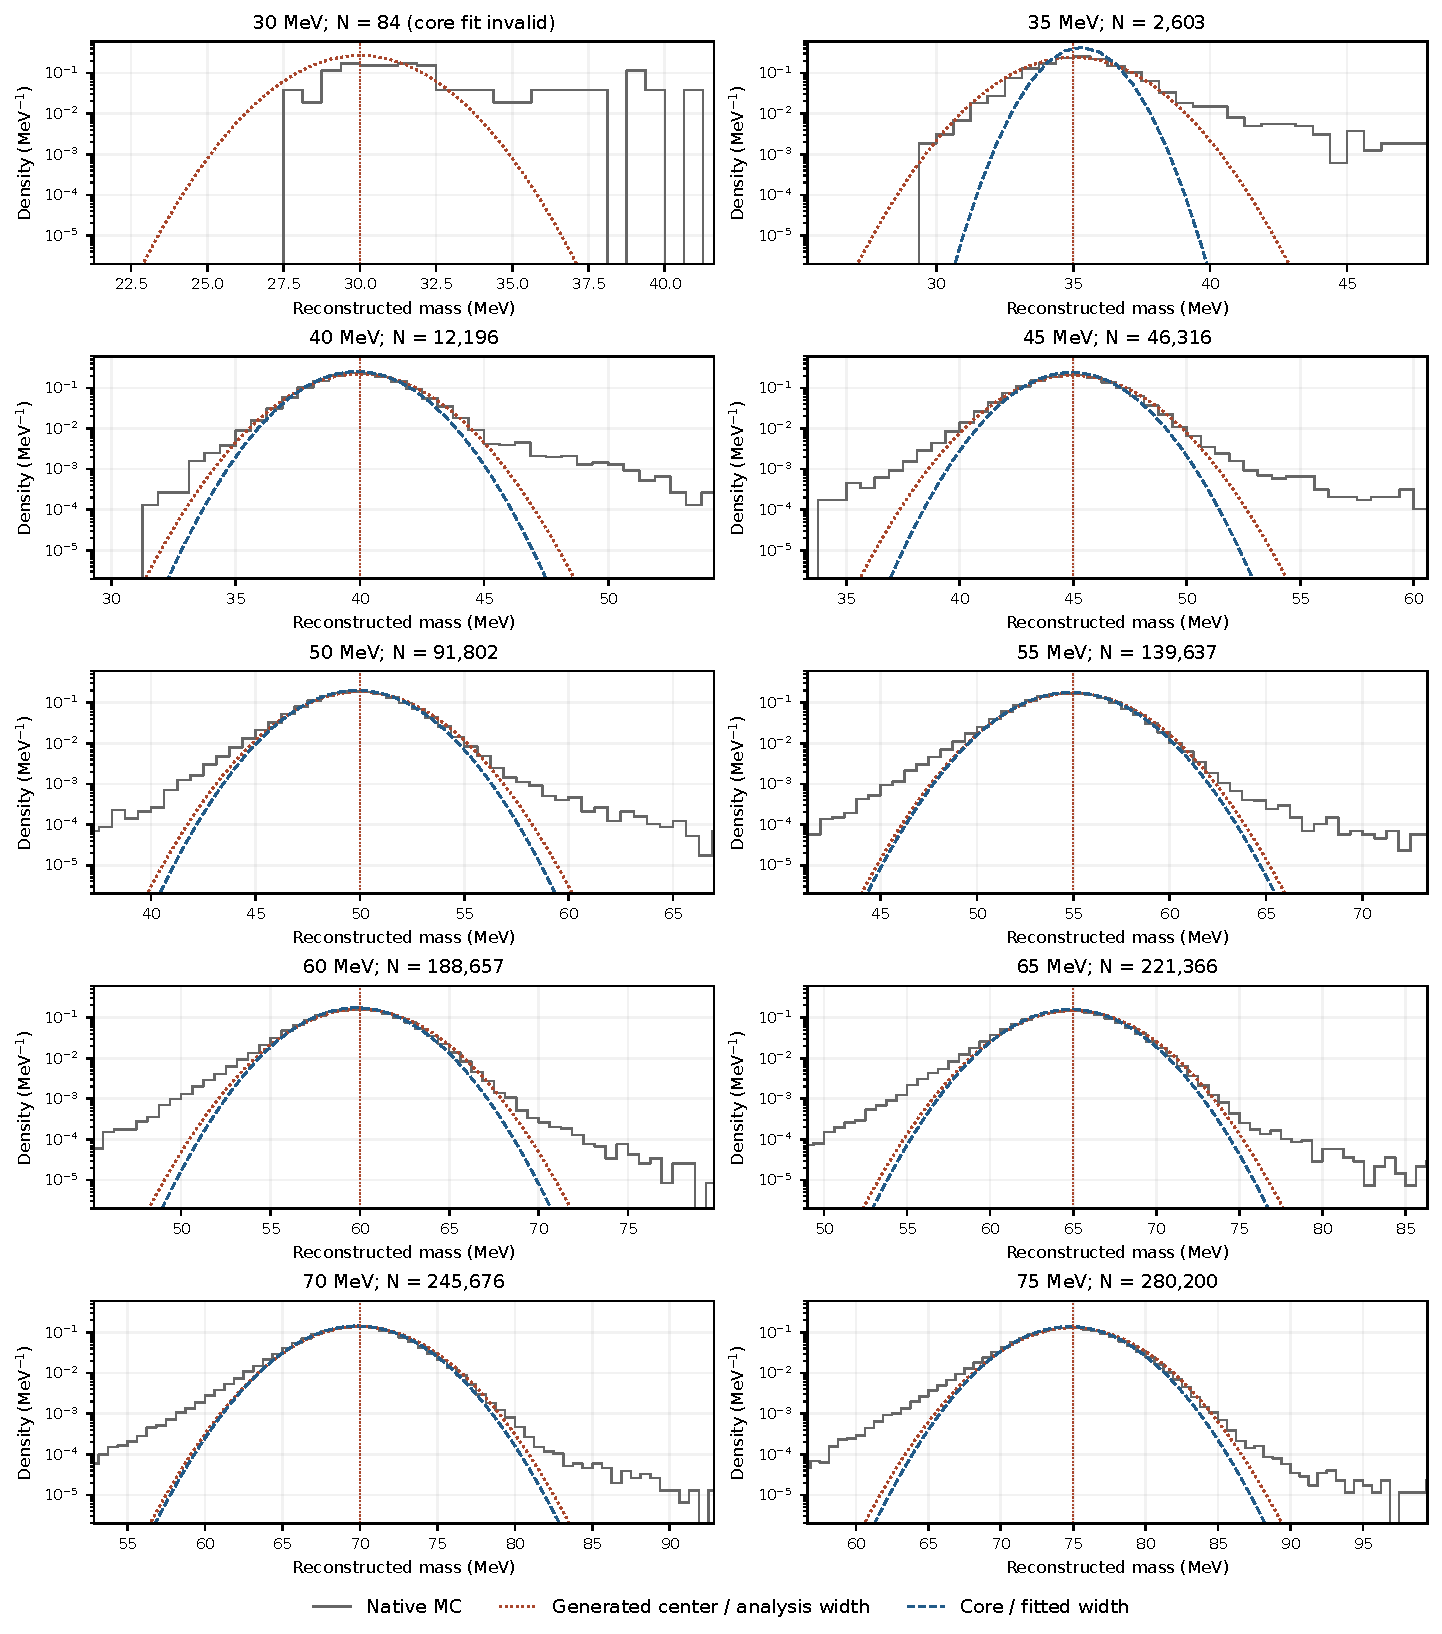
\includegraphics[width=\linewidth,height=6.65in,keepaspectratio]{../figures/shape_catalogue_1.pdf}\end{center}
{\small\refstepcounter{figure}\textbf{Figure \thefigure. How to read the figure.} Each panel shows the native MC with full selected normalization. Red dotted: a unit-area Gaussian at the generated mass with the reference analysis width. Blue dashed: a unit-area Gaussian at the fitted core with its fitted width. They are comparison shapes, rather than the local Gaussian component plus pedestal shown earlier. No blue curve is shown for the invalid 30 MeV core. The logarithmic axis exposes tails, and the displayed range does not change the normalization.}\par\medskip

\clearpage\section*{Native signal-MC catalogue: 80--125 MeV}
\begin{center}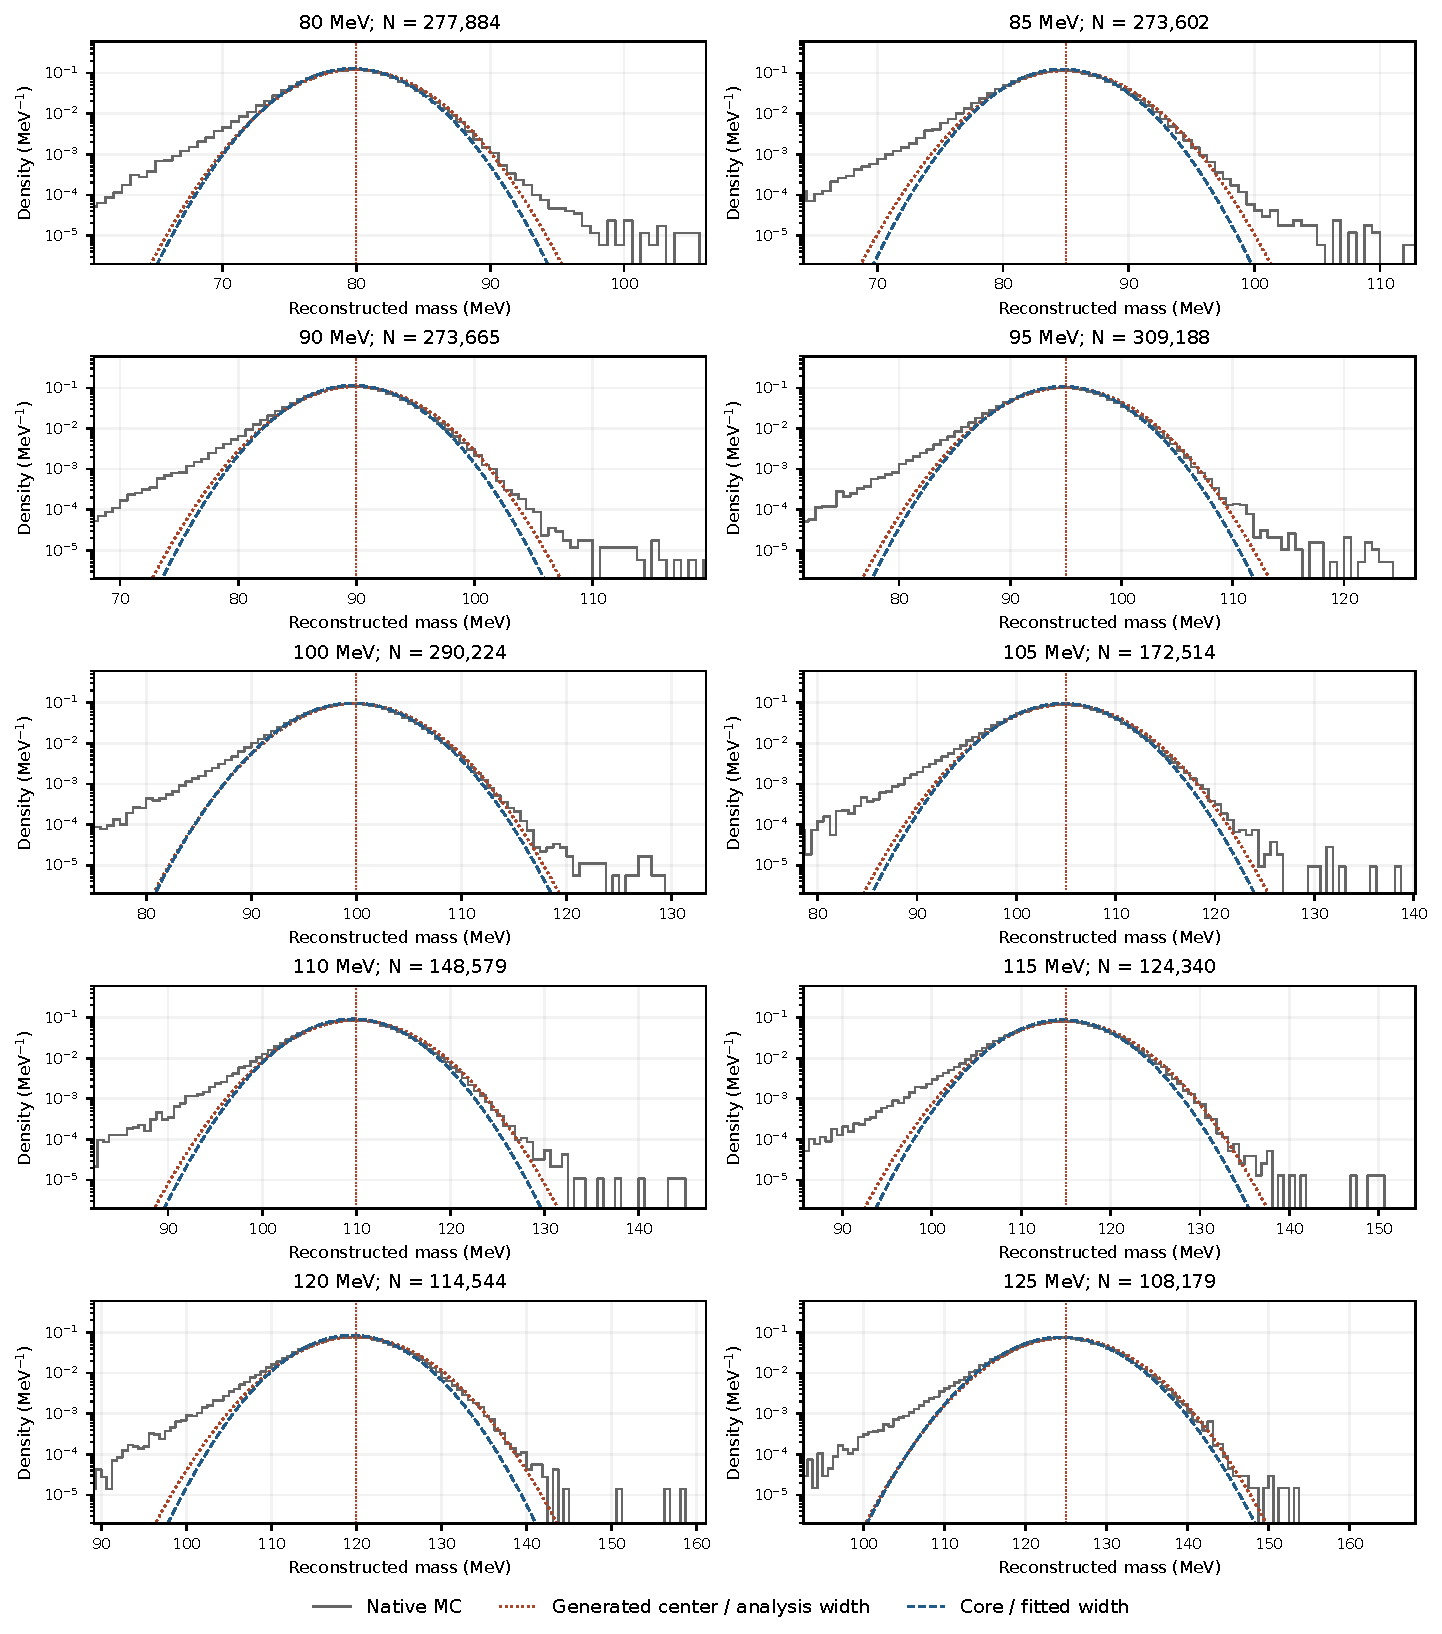
\includegraphics[width=\linewidth,height=6.65in,keepaspectratio]{../figures/shape_catalogue_2.pdf}\end{center}
{\small\refstepcounter{figure}\textbf{Figure \thefigure. How to read the figure.} Gray: native MC. Red dotted: Gaussian at the generated mass with the reference analysis width. Blue dashed: Gaussian at the fitted core with its fitted width. Both Gaussians have unit full area. The logarithmic scale reveals shoulders and tails that are less visible on a linear scale. The empirical MC template used for extraction retains those features; the Gaussians provide visual comparisons.}\par\medskip

\clearpage\section*{Native signal-MC catalogue: 130--175 MeV}
\begin{center}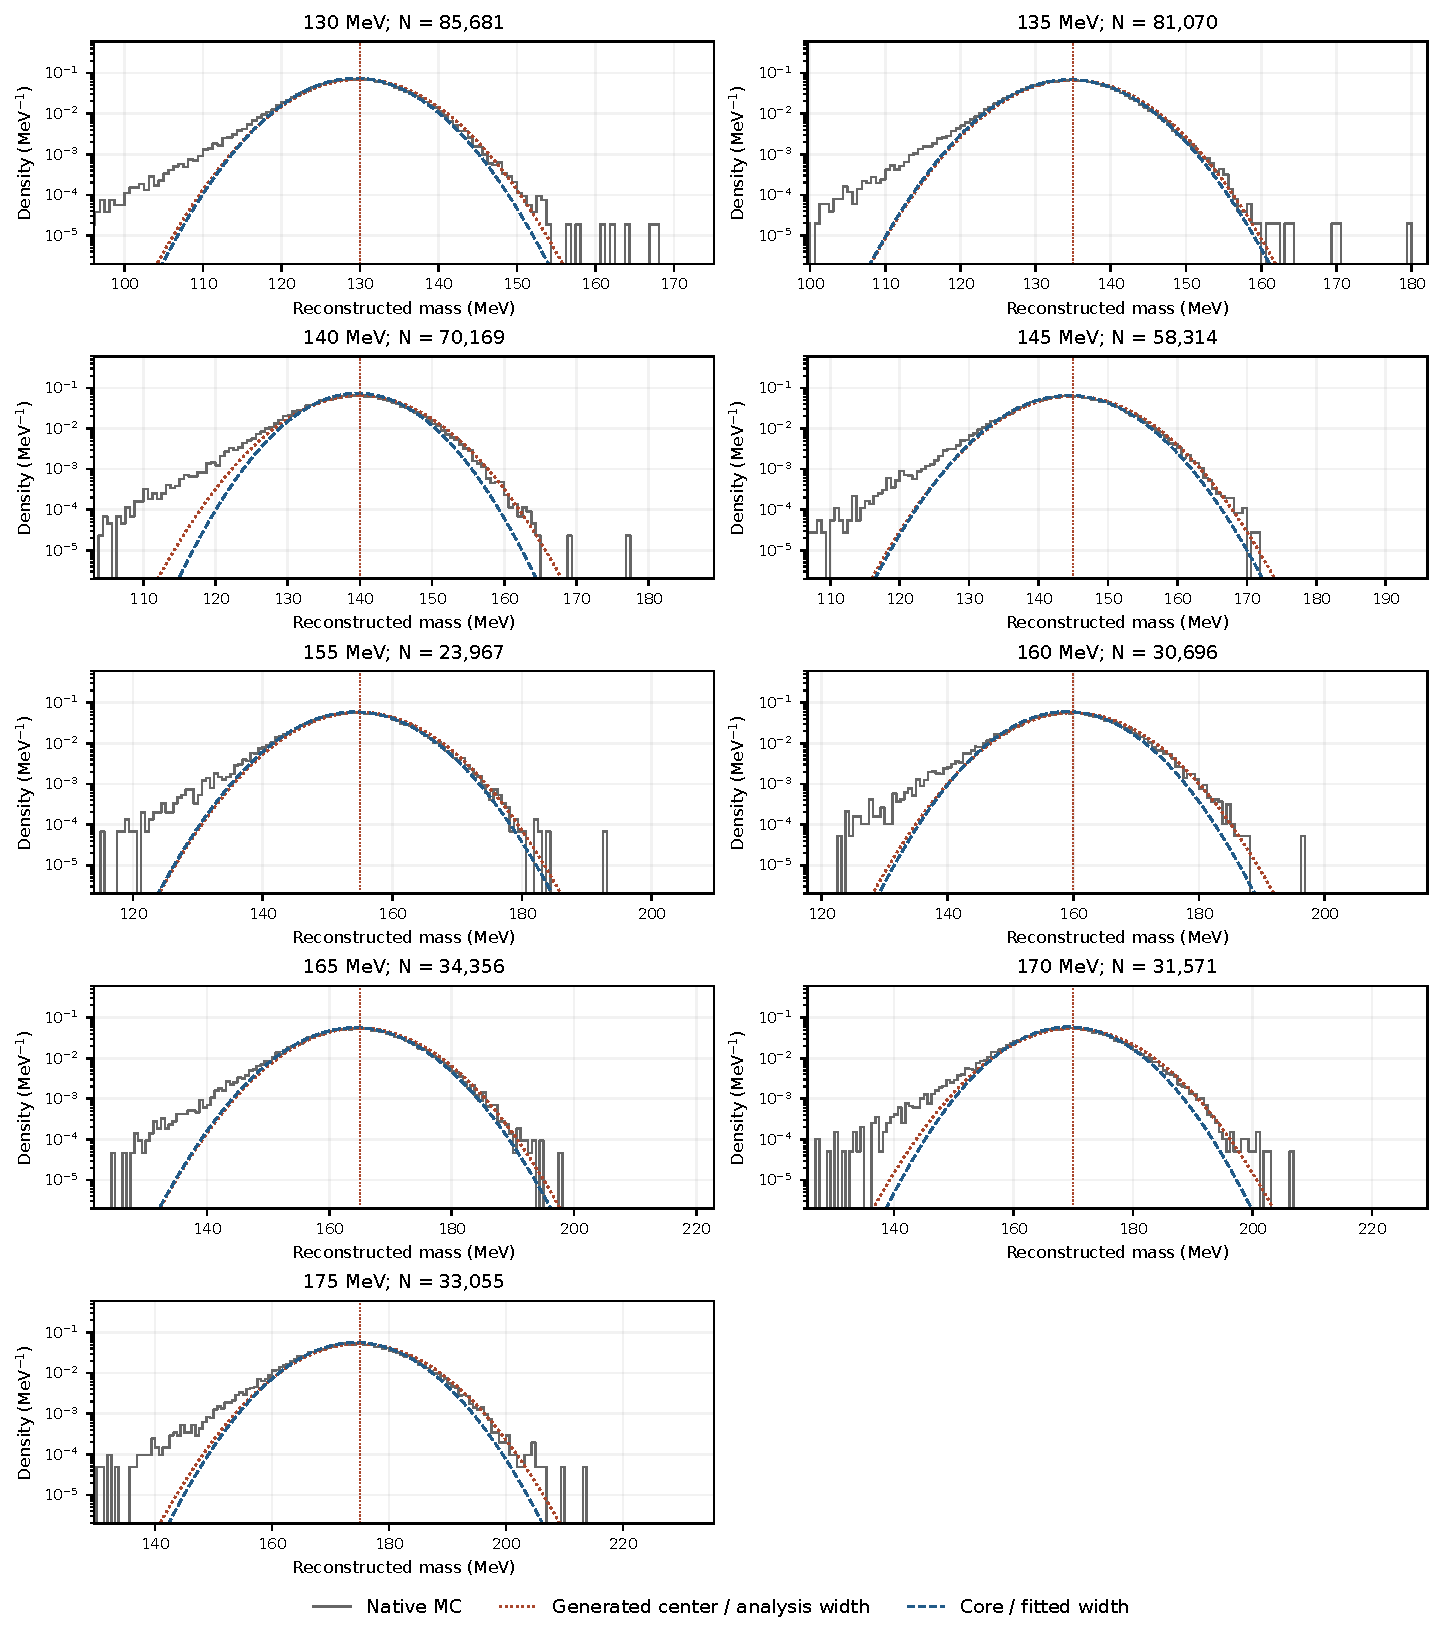
\includegraphics[width=\linewidth,height=6.65in,keepaspectratio]{../figures/shape_catalogue_3.pdf}\end{center}
{\small\refstepcounter{figure}\textbf{Figure \thefigure. How to read the figure.} Gray: native MC. Red dotted: Gaussian at the generated mass with the reference analysis width. Blue dashed: Gaussian at the fitted core with its fitted width. The available inputs jump from 145 to 155 MeV; no simulated 150 MeV histogram is shown. All displayed densities retain their full selected normalization. The high-mass center errors and definition spreads are listed in the preceding table.}\par\medskip
